%\gbt{Points to discuss in the paper, as discussed with Carina May 16:}
%
%\begin{itemize}
%\item Super high variance in the agreement. Higher agreement for instances, lower for classes. Suggests systematicities at the instance level that do not depend on the class. Hypothesis, supported by qualitative analysis (Figure 3): relevance of visual perceptual factors. E.g.: saliency, background/foreground (desk-keyboard; bridge-train); ``angle'' from which the object is shown (see girl-t-shirt example); \dots In addition, we also find aspects discussed by Psycholing, but at the level of the instance: Typicality (see truck-bus example, bridge-dock, bench-seat). 
%\item Forget about WordNet.
%\item Implications for lang\&vision: 1) synset classification won't do (if the goal is to predict/label an object); 2) name classification won't do either; 3) ``mistakes'' done by models are also done by humans -- role of referential uncertainty.
%\end{itemize}

We investigate to what extent names in VisualGenome (\vg) and ManyNames can be considered canonical.%, i.e., to what extent speakers agree in their naming choices.
Whereas traditional picture naming studies typically use a prototypical image per category (see Figure~\ref{fig:picture_naming}) and, hence, look at concept-level agreement, we examine to what extent names overlap (i) for the same object and (ii) for different instances of the same class, based on the canonicalized names in \vg.

\subsection{Names, Instances, Classes}
\label{subsec:counts}

We analyse the following annotations associated with each object: (i) the original name, annotated in \vg, (ii) the object class or synset, annotated in \vg and obtained via a semi-automatic linking of the object name to WordNet\footnote{Recall that we used these VG synsets for collecting our images (Section~\ref{ssec:sampling})}, (iii) the ManyNames response set, i.e. a set of name types with annotation frequencies (max. 36 annotations per object). See Figure \ref{fig:ex-high-low-agreement} for examples of objects and their response sets (top rows below the images).
 %[if model preds are kept]}. 
 Based on the \vg synsets, we aggregate the annotations for instances of the same class and obtain a class-level response set that contains all names and their frequencies annotated for all objects of a class. 
 
% As a first simple measure of variation in object naming, we simply count how many different names (i.e.\ types) are given to instances and to classes.
%Since a certain amount of noise in the crowd-sourced ManyNames data can be expected, we explore different frequency thresholds (from 1 to 6) to filter the response sets.
Figure \ref{fig:ntypes} shows the cumulative histograms for type counts, i.e.\ how many objects (left) or classes (right) have at least $n$\ names, with different frequency thresholds~$n$ to account for possible noise in the crowdsourced data.
Without any frequency thresholding~\mbox{($n$=1)}, the proportion of instances and classes that have a single name annotated is very small, below 10\%\ in both cases. 

The histogram for instances in Figure\ \ref{fig:ntypes} suggests that there is a certain amount of low-frequency responses in the ManyNames data, as is expected in an annotation task where subjects are free to choose any response. 
When discarding names with frequencies below\ \mbox{2, 3 or 4}, the %response sets for instances get more consistent such that the majority contains at most 5\ names.
majority of the response sets for instances become more consistent with at most 5\ names per set, 
%Nevertheless, the proportion of objects that really only have a single name annotated is still below 50\%. %, even when applying a strict frequency filter of 4.
but the sets with a single name still make up only $<$50\%\ of all sets. 
In sum, this indicates that there is non-negligible variation when different speakers name the same object, and the variation seems to be restricted to a manageable set of up to 5\ names per object.

However, the number of types increases substantially when aggregating responses over classes, as shown in the cumulative histogram for type counts of synsets in Figure\ \ref{fig:ntypes}\ (right).
%Here, we observe that the 
The rise of the curve is much less steep than for instances and, generally, there are many synsets with more than 10\ or even 20\ different name types, even after applying the frequency thresholds. This clearly indicates that different instances annotated with the same 
%name and 
\cs{(removed "name and") The synsets could have different names -- maybe say "or even same name"?}
synset in \vg trigger different naming variants. Examples illustrating this can be found in Figure \ref{fig:ex-high-low-agreement}. 
Implications of this finding will be discussed below in Section \ref{subsec:discuss}.

\begin{figure*}
\begin{minipage}[b]{0.4\linewidth}
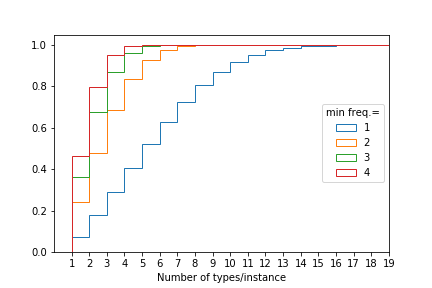
\includegraphics[scale=.4]{figures/types_instances.png}
\end{minipage}
\begin{minipage}[b]{0.6\linewidth}
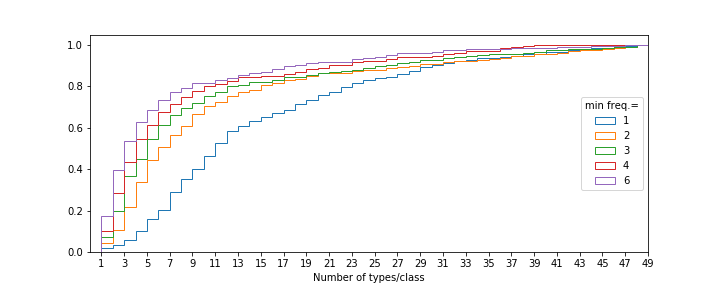
\includegraphics[scale=.4]{figures/types_classes.png}
\end{minipage}
 \caption{\label{fig:ntypes} Cumulative histograms for number of types found for instances and classes, based on different frequency tresholds (applied on the level of instances and classes respectively)}
\end{figure*}
\cs{Change yticks to 0-100, with label \%. Make font larger in Fig. with plots?}

\begin{table*}
\footnotesize
%\begin{tabular}{p{1.3cm}cccccc|cccccc}
%\toprule
% & \multicolumn{6}{c|}{Instance-level agreement} & \multicolumn{6}{c}{Class-level agreement}\\ 
%           domain & \% top &    $H$ &    N & N$_{>1}$ & top=VG &  \% VG & \% top &    $H$ &     N & N$_{>1}$ & top=VG &  \% VG \\
%\midrule
%            all &  69.7 (22.2) &  1.3 &  5.7 &   2.9 &  72.8  &  58.7  &   52.6 (21.1) &  2.4 &   62.2 &  29.7 &  32.7 (46.9) &  23.5 (27.0)  \\
% \midrule
%         people &  51.9 (18.1) &  2.1 &  8.6 &   4.3 &         49.8 &         32.3 &     43.1 (14.9) &  2.9 &  104.4 &  53.4 &         24.4 &         13.2  \\
% animals\_plants &  91.3 (12.9) &  0.4 &  2.7 &   1.5 &         93.8 &         88.0 &     67.9 (23.5) &  1.5 &   26.7 &  12.4 &         29.5 &         26.2  \\
%       clothing &  63.9 (17.9) &  1.6 &  6.4 &   3.2 &         70.2 &         52.6 &     49.3 (16.6) &  2.6 &   71.7 &  34.1 &         40.5 &         26.1  \\
%       vehicles &  72.0 (19.5) &  1.1 &  4.7 &   2.4 &         71.1 &         60.2 &    54.4 (17.4) &  2.1 &   70.4 &  33.2 &         21.4 &         21.3  \\
%      buildings &  66.9 (20.5) &  1.5 &  6.9 &   3.0 &         72.6 &         55.5 &      46.7 (18.2) &  3.0 &   68.5 &  31.3 &         32.3 &         22.3  \\
%           home &  66.4 (20.5) &  1.5 &  6.3 &   3.1 &         78.5 &         58.8 &     49.6 (18.7) &  2.8 &  103.2 &  48.8 &         45.9 &         30.1  \\
%           food &  71.3 (21.1) &  1.3 &  5.5 &   2.9 &         62.9 &         52.1 &     47.3 (19.5) &  2.5 &   32.1 &  15.2 &         31.1 &         20.8  \\
%\bottomrule
%\end{tabular}

\begin{tabular}{lccccc|ccccc}
\toprule
 & \multicolumn{5}{c|}{Instance-level agreement} & \multicolumn{5}{c}{Class-level agreement}\\ 
          domain &    N &         \%top (std) &          H (std) & top=VG &   \%VG &     N &         \%top (std) &          H (std) & top=VG &   \%VG \\
\midrule
            all &  2.9 &  75.2 (21.9) &  0.9 (0.7) &   72.8 &  62.8 &  29.7 &  56.4 (21.5) &  2.0 (1.0) &   32.7 &  23.4 \\
            \midrule
                     people &  4.3 &  59.0 (20.4) &  1.5 (0.7) &   49.8 &  36.3 &  53.4 &  47.5 (17.2) &  2.5 (0.9) &   24.4 &  13.0 \\
       clothing &  3.2 &  70.1 (18.5) &  1.1 (0.6) &   70.2 &  57.4 &  34.1 &  53.4 (16.6) &  2.1 (0.8) &   40.5 &  26.1 \\
           home &  3.1 &  72.6 (20.7) &  1.0 (0.7) &   78.5 &  64.1 &  48.8 &  54.0 (19.4) &  2.3 (1.0) &   45.9 &  29.9 \\
                 buildings &  3.0 &  74.7 (20.7) &  1.0 (0.7) &   72.6 &  61.6 &  31.3 &  51.0 (18.8) &  2.4 (0.9) &   32.3 &  22.2 \\
           food &  2.9 &  76.4 (20.7) &  0.9 (0.7) &   62.9 &  55.2 &  15.2 &  50.8 (20.3) &  2.0 (0.8) &   31.1 &  20.8 \\
                  vehicles &  2.4 &  76.6 (19.8) &  0.8 (0.6) &   71.1 &  63.9 &  33.2 &  57.4 (17.3) &  1.8 (0.6) &   21.4 &  21.2 \\
 animals\_plants &  1.5 &  94.5 (12.1) &  0.2 (0.4) &   93.8 &  91.0 &  12.4 &  71.3 (23.3) &  1.2 (0.9) &   29.5 &  26.1 \\
\bottomrule
\end{tabular}

\caption{Agreement in naming measured on the level of instances and on the level of \vgenome classes (i.e.\ after grouping objects by their \vg synset), for filtered response sets (frequency threshold of 2)}
\label{tab:agree}
\end{table*}

\subsection{Agreement}

%As type counts give a rather rough indication for variation in object naming, 
We compute the following measures to assess agreement on the object names:
\begin{itemize}
\item \textbf{\% top}: the average relative frequency of the most frequent response (shown in percent)
\item \textbf{$H$}: the $H$ agreement measure from \citet{snodgrass}, where 0 is perfect agreement: \mbox{$H = \sum_{i=1}^k p_i~log_2\frac{1}{p_i}$}, 
where $k$\ denotes the number of name types and $p_i$\ is the proportion of name type\ $i$ in the response set. \cs{@Sina: right?}

% \begin{equation}
% H = \sum_{i=1}^k p_i\ log_2(1/p_i)
% \end{equation}

\item \textbf{N}: the average number of types in the response set of ManyNames
\item \textbf{top=VG}: the proportion of items where the top response in ManyNames corresponds to the \vg name \cs{the numbers are percentages, aren't they? So we should either say "relative frequency", leaving open that we express it as percentage, or directly percentages. Proportion should be a value between 0 and 1, shouldn't it?!}
\item \textbf{\% VG}: the average relative frequency of the \vg name in the response set 
\end{itemize}
\cs{Maybe it would be good to give an example for the class-level, to make it easier to follow the results discussion}
Again, we measure instance-level and class-level agreement on response sets for objects and synset classes, respectively.
To account for potential noise\cs{redundant}, we filter out names with a frequency of\ 1 from the response sets.

As shown in Table\ \ref{tab:agree}, generally, the agreement measures follow a similar pattern as the type counts discussed in Section\ \ref{subsec:counts}:
On the instance level, our annotators achieve a fair amount of overlap in their object naming choices, with the most frequent name accounting for 75\%\ of the responses on average, and the original \vg name having an average frequency of\ 63\% in the ManyNames responses. On the class level, however, the agreement is much lower: The average frequency of the top name drops to\ 56\% and that of the \vg name even to\ 23\%. The $H$ measures indicate a fair amount of agreement for instances, a bit lower than the agreement found in picture norming studies on artificial images (e.g.\ \newcite{snodgrass} report an average $H$ of 0.55). On the class-level, again, an average $H$ value of 2 points to a much more even distribution of name frequencies.

%Generally, this seems to suggest that indeed many objects in our data set have a canonical name. 
%\sz{For NLP people, this looks like a good agreement (given that people were free to type what they wanted). For vision people who might think of it as an object labeling task, this would be pretty low/bad agreement.}
%At the same time, the average number of name types per object (5.7, or 2.9 when excluding low-frequency types in each response set) suggests that there is a stable amount of naming variants that is elicited for instances. 
If we check agreement by domain, two domains stand out: the \textsc{animals,plants} domain, which is often discussed in the object naming literature and where we find almost perfect agreement\ (\mbox{$H=0.2$}), and the \textsc{people} domain with a particularly low agreement.
In the other domains values are around the average for the whole dataset\cs{remove because redundant?}.
%For the other domains the $H$ value ranges around 1, and \%top is between 70\% and 80\%.

Another important aspect however is the large standard deviation values for both \%top and $H$, that we find both when averaging over all objects and within objects of the same domain \cs{redundant--it is true for each case}. This indicates that the agreement varies a lot across instances\cs{", which shows that there is a high variance in agreement"(?)}, over and above the class or domain\cs{??}.
The qualitative examples in Figure \ref{fig:ex-high-low-agreement} %further corroborate this evidence: depending on the visual instance, the agreement can be very high or very low.
illustrate this, showing visual instances with very high or low agreement. 
These examples suggest that instances which are more prototypical of a category trigger higher agreement.
The following section will examine other potential sources of variation in object naming.


\subsection{Specificity and Other Sources of Variation}
\label{ssec:variation}
Previous work on object naming has mostly adopted taxonomy-driven models aimed at capturing objects names of different levels of specificity~\cite{+++}.
%This section shows that naming variation in ManyNames cannot be explained by this parameter.
This parameter does not explain the naming variation in ManyNames, as we will show in the following. 
Given that the \vg names are already linked to WordNet synsets, we compute the same linking for the additional ManyNames names, and examine whether they stand in a taxonomic relation to the objects'  \vg  synsets.% given by \vg.
%%In this section, we take a closer look at the lexical variation we observe in our data set. 
%We analyze the data points where participants attributed different names to the same object and extract a set of  pairwise \textbf{naming variants}. These naming variants correspond to pairs of words that can be used interchangeably to name certain objects.
%For each object, we extract the set of naming variants $s = \{ (w_{top},w_2), (w_{top},w_3), (w_{top},w_4),... \}$  where $w_{top}$ is the most frequent name annotated for the object and $w_2 ... w_n$ constitute the less frequent alternatives of $w_{top}$.  The  \textbf{type frequency} of a naming variant $(w_{top},w_x)$ corresponds to the number of objects where this variant occurs. The \textbf{token frequency} of $(w_{top},w_x)$ corresponds the count of all annotations where $w_x$ has been used instead of $w_{top}$.
%In Table \ref{tab:exvariants}, we show the naming variants with the highest raw token frequency for each domain. 
%The naming variants can be grouped according to their lexical relation, as follows:
%
%\begin{itemize}
%\item \textbf{synonymy}: e.g.\ aircraft vs. airplane 
%\item \textbf{hyponymy}: e.g.\ man vs. person
%\item \textbf{co-hyponymy}: e.g.\ swan vs. goose
%\item \textbf{no relation}: e.g.\  desk vs. apple
%\end{itemize}
\cs{Shouldn't we mention that we consider only simple move-up hypernymy relations?}
Table \ref{tab:rel} shows the distribution of the results. 
how frequently names with a certain relation to the synset occur in the aggregated class-level response set, in terms of their  type and token frequency. 
\cs{something went wrong here --- "(?)Table\ \ref{tab:rel} shows the relative frequency distribution of the relations (between the MN names %types and tokens, respectively, 
and the VG synsets) in the aggregated class-level response sets." // "Table \ref{tab:rel} shows the relative frequency distribution of the different relations which occur between the MN names and the VG synsets in the aggregated class-level response sets."} 
\gbt{what do you mean, `` aggregated class-level response set''?}
\cs{Considering the track we are submitting to, one or two examples per relation in an additional column in the table wouldn't hurt.}
The coverage of WordNet for our name data is satisfactory (90\%\ of the name types, accounting for 97\%\ of the tokens).
Among the names that do have a hierarchical relation to the synset, hypernyms are the most frequent, meaning that our annotators often went for a more general name than the \vg annotators.
However, in the vast majority of cases no hierarchical relation between the name and the synset can be retrieved from WordNet.
Thus, strikingly, most of the naming variation in ManyNames is \textit{not} related to different preferences in levels of specificity, %\cs{(as far as it can be determined using WordNet)}
 but to other sources.

\begin{table}
\small
\centering
\begin{tabular}{lcc}
\toprule
         relation & \% types & \% token \\
\midrule
% meronym &  0.1 &  0.2 \\
% holonym &  0.1 &  0.4 \\
 word-not-covered &  10.6 &  2.6 \\
\midrule
 synonym &  1.1 &  1.1 \\
 hyponym &  2.2 &  3.8 \\
 co-hyponym &  3.1 &  5.9 \\
 hypernym &  10.5 &  27.7 \\
 rel-not-covered &  72.2 &  58.3 \\
\bottomrule
\end{tabular}
\caption{Lexical relations of naming variants in ManyNames to annotated \vg synset, averaged over synsets.}
\label{tab:rel}
\end{table}

We discuss other types of variation we found in the data, based on qualitative analysis, and illustrate them with the examples in Figure\ \ref{fig:ex-high-low-agreement}:

\begin{description}
\item[Referential uncertainty:] despite our care in filtering out objects that are occluded or have unclear bounding boxes (see\ Section~\ref{sec:data}), we still find many examples where annotators identified different objects for the same bounding box. They typically named an adjacent object or one supported by the target object (e.g.\ \textit{book-bed}) or a part of the target object (\textit{pants-player}).
Note that, while some of these cases are arguably annotation errors (\textit{boy-helmet}), in many cases it is not possible to distinguish which object is being indicated (\textit{bed-sleeping bag}). Pointing gestures in natural communication are as referentially uncertain as bounding boxes; however, typically those gestures are grounded in a specific discourse context, which helps reduced uncertainty.
\item[Cross-classification:] a substantial group is constituted by names conceptualizing alternative aspects of the same object (e.g. \textit{boy-batter}, \textit{dessert-toast}).
\item[Conceptual disagreement:] as we did not filter objects for prototypicality, our data mirrors a certain amount of disagreement between speakers (\textit{bed-bench}, \textit{sandwich-hotdog})
\item[Metonymy:] similar to cross-classification, we find examples reminiscent of metonymy discussed in the linguistic literature \cite{pustejovsky1991generative} where logically related parts of an object stand in as its name (\textit{sandwich-basket}, \textit{bed-bed sheet}). 
\item[Issues with WordNet:] due to WordNet's fine-grained hierarchy, it is difficult to retrieve certain loosely related synonyms or hypernyms (\textit{robe-dress}).
\end{description}

As it is non-trivial to separate this cases, we leave a precise quantitative analysis of these phenomena for future work.

%\begin{table}
%\small
%\begin{tabular}{lp{4.8cm}r}
%\toprule
%VG name &  top5 MN names &  n$_{obj}$  \\
%\midrule
%\multicolumn{3}{c}{\it Canonical VG names with max agreement in MN}\\
% giraffe &  giraffe (96.8), animal (1.2), zebra (0.4), camel (0.3), pole (0.1) &  915 \\
% zebra &  zebra (96.3), animal (1.0), giraffe (0.9), horse (0.2), microwave (0.2) &  461  \\
% cat &  cat (94.8), animal (0.9), kitten (0.8), dog (0.4), laptop (0.2) &  754\\
%\midrule
%\multicolumn{3}{c}{\it Canonical VG names with min agreement in MN}\\
% booth &  booth (19.3), table (12.3), phone booth (9.8), bench (6.7), building (4.4) &  11 \\
% cabbage &  cabbage (21.4), lettuce (17.0), hotdog (11.9), food (10.7), salad (10.4) &  9 \\
% robe &  robe (22.1), shirt (16.8), jacket (13.3), dress (5.7), clothing (3.2) &  19 \\
%  \midrule
%  \multicolumn{3}{c}{\it Non-canon. VG names with max agreement in MN}\\
% sedan &  car (88.4), wheel (3.1), vehicle (2.3), automobile (1.3), dog (0.8) &  11 \\
% pony &  horse (83.9), pony (9.1), animal (2.9), donkey (1.1), cow (1.1) &  8 \\
% necktie &  tie (81.4), necktie (10.2), shirt (4.6), ties (1.5), jacket (0.5) &  11 \\
% \midrule
%   \multicolumn{3}{c}{\it Non-canon. VG names with min agreement in MN}\\
% shelter &  umbrella (9.7), shelter (8.8), roof (8.0), tent (7.1), building (6.8) &  10 \\
% bath &  shower (13.3), elephant (9.9), birdbath (8.1), water (7.2), trough (7.2) &  10 \\
% vegetable &  food (15.7), broccoli (13.1), sandwich (10.6), salad (9.3), pizza (7.8) &  25 \\
%\bottomrule
%\end{tabular}
%\caption{Examples for VisualGenome (VG) names and their most frequent corresponding responses in ManyNames (MN; percentages shown in brackets). ``Canonical'' means that the VG name is the top name in MN, and non-canonical vice versa.}
%\label{tab:qual}
%\end{table}
\begin{figure*}[t]
	\begin{minipage}[b]{0.5\linewidth}
		{\scriptsize
			\setlength{\tabcolsep}{1pt}
			\begin{tabular}{p{2.6cm}|p{2.6cm}|p{2.6cm}|p{2.6cm}|p{2.6cm}|p{2.6cm}}
				%\textbf{desk} &  \raisebox{-\totalheight}{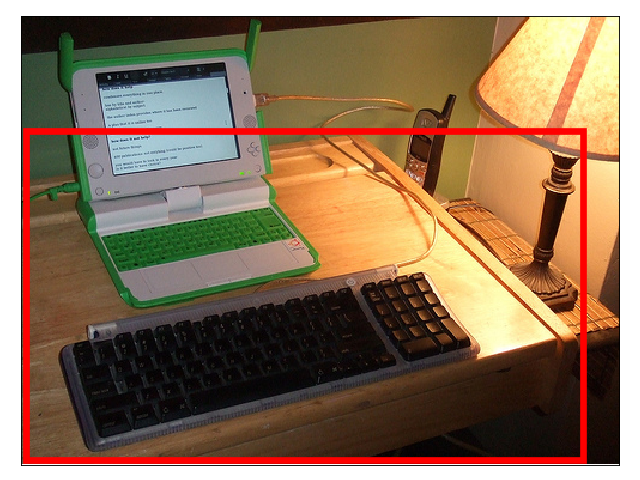
\includegraphics[width=0.9\linewidth]{figures/2320949_1048853_singleton_obj.png}} MN: keyboard  &
				%\raisebox{-\totalheight}{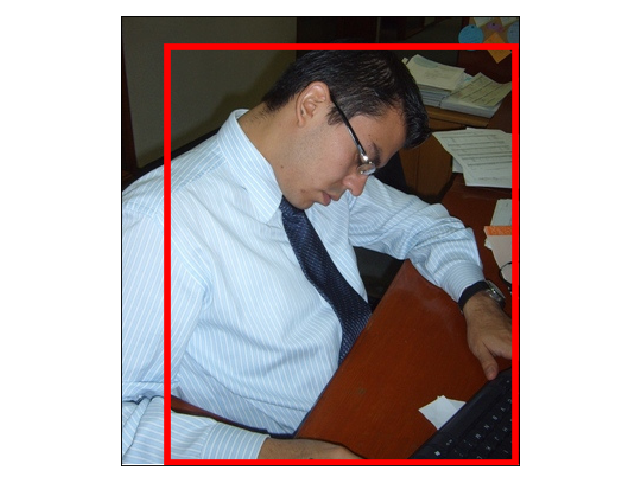
\includegraphics[width=0.9\linewidth]{figures/2343219_926143_supercat_unique.png}}  MN: desktop &
				%\raisebox{-\totalheight}{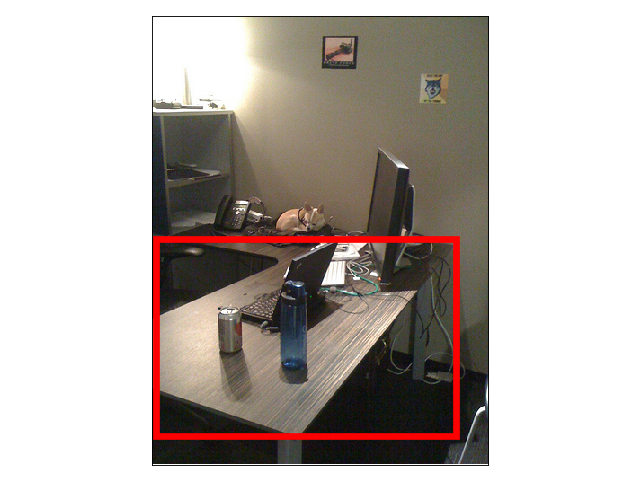
\includegraphics[width=0.9\linewidth]{figures/2354847_1742687_seed_ambiguous.png}} MN: computer \\
				%\textbf{bench} &  \raisebox{-\totalheight}{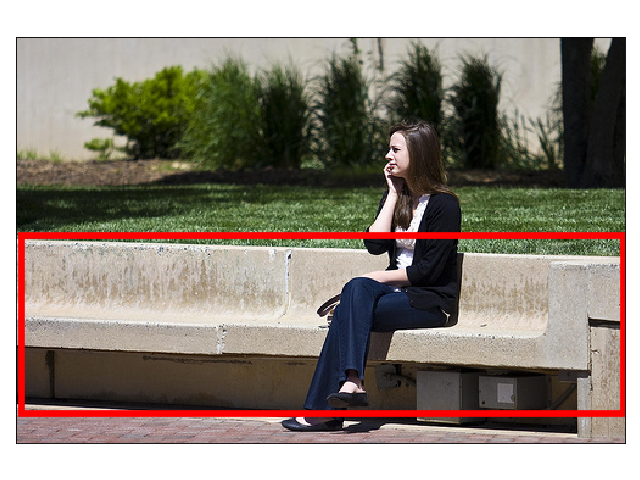
\includegraphics[width=0.9\linewidth]{figures/2350360_1042111_supercat_unique.png}} MN: table  &
				%\raisebox{-\totalheight}{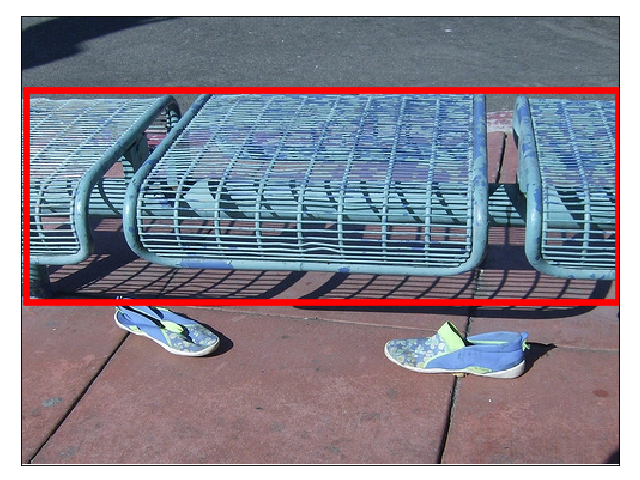
\includegraphics[width=0.9\linewidth]{figures/2389358_1261752_singleton_obj.png}}  MN: seat &
				%\raisebox{-\totalheight}{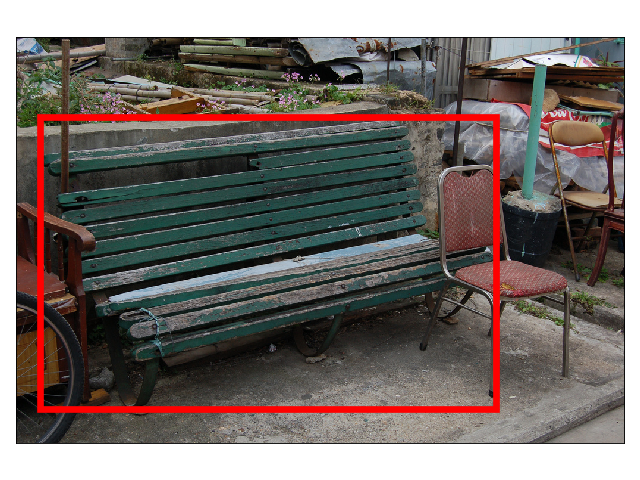
\includegraphics[width=0.9\linewidth]{figures/1593011_2063521_singleton_obj.png}} MN: wood \\
				\multicolumn{4}{c|}{\textbf{VG: sandwich}} & \multicolumn{2}{c}{\textbf{VG: robe}}\\
				\raisebox{-\totalheight}{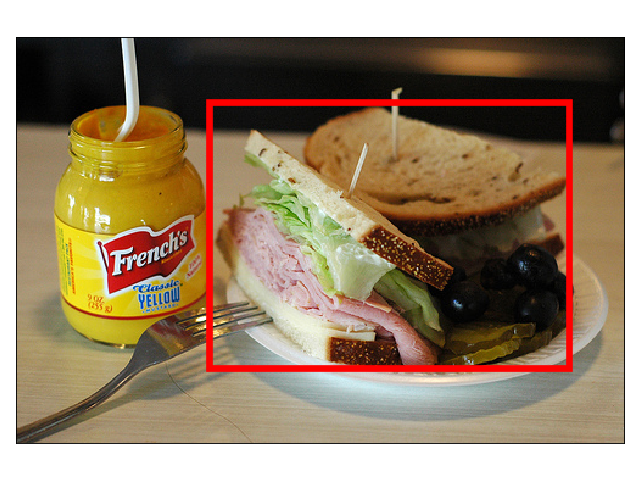
\includegraphics[width=0.9\linewidth]{figures/2339876_3928476_supercat_unique.png}} sandwich (34) &
				\raisebox{-\totalheight}{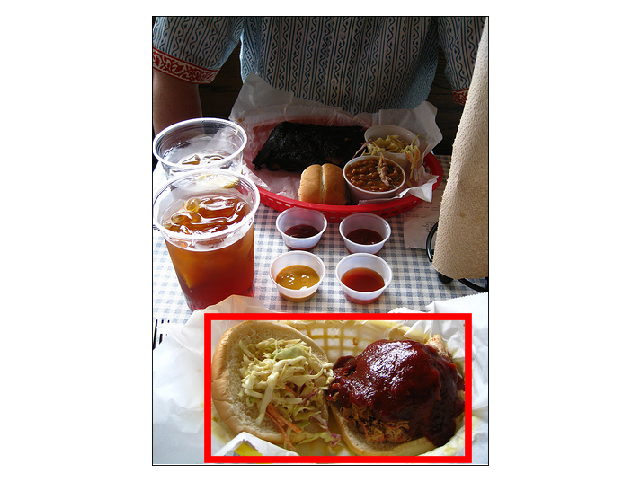
\includegraphics[width=0.9\linewidth]{figures/2379889_1353176_supercat_unique.png}}  sandwich (15), basket (6), \underline{food} (5), burger (2),  \underline{hamburger} (2),  \underline{meal} (2) &
				\raisebox{-\totalheight}{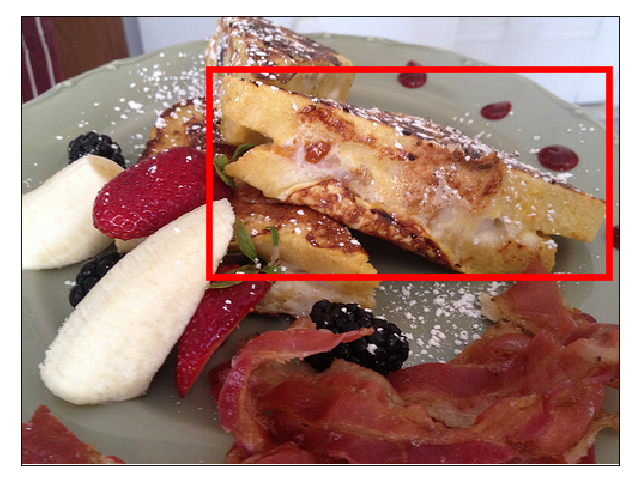
\includegraphics[width=0.9\linewidth]{figures/2394266_465678_singleton_obj.png}} \underline{food} (10), sandwich (8), toast (5), french toast (4), dessert (2), breakfast (2) &
				\raisebox{-\totalheight}{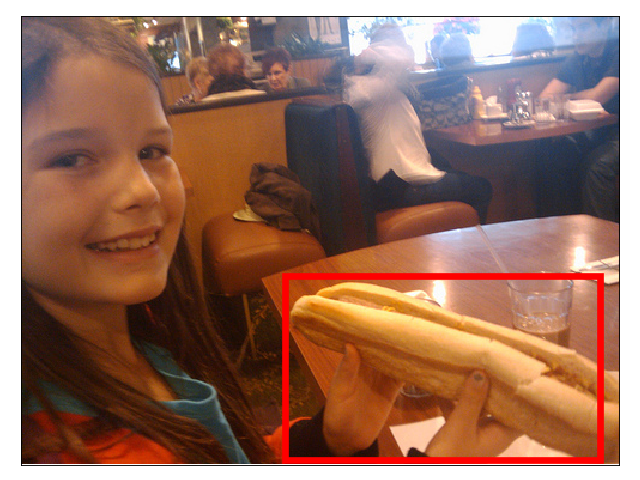
\includegraphics[width=0.9\linewidth]{figures/2386509_681763_supercat_unique.png}} hotdog (14), \underline{food} (7), bun (4), sandwich (3),  \underline{bread} (2) [banana (1)] &
				\raisebox{-\totalheight}{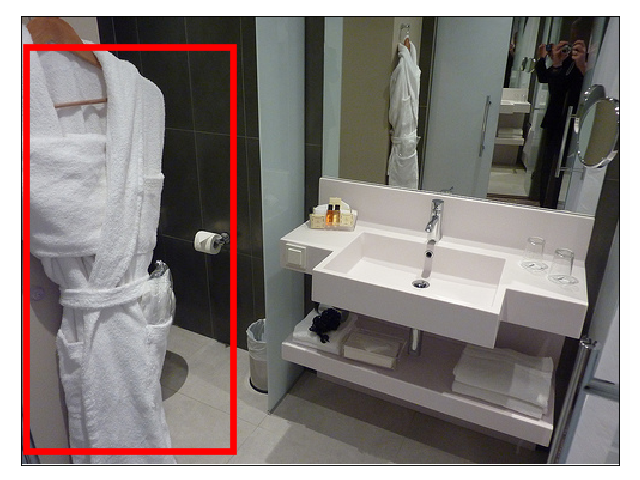
\includegraphics[width=0.9\linewidth]{figures/2373180_2333161_singleton_obj.png}} robe (27), \underline{bathrobe} (5) &
				\raisebox{-\totalheight}{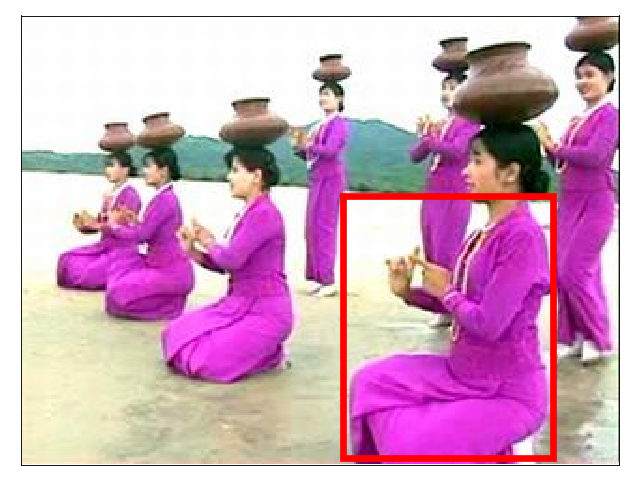
\includegraphics[width=0.9\linewidth]{figures/160_1058761_supercat_unique.png}} dress (30), uniform (2)\\ 
				%
				\rowcolor{lightgray}
				 \textit{sandwich}, food, bread, sandwiches, plate, burger
				 & plate, \textit{food}, \textit{basket}, hotdog, wrapper, paper
				 & fish, chicken, meat, \textit{food}, \textit{sandwich}, bread
				 & \textit{hotdog}, \textit{bun}, \textit{banana}, \textit{bread}, table
				 & woman, outfit, dress, girl, suit
				& woman, outfit, \textit{dress}, girl, suit \\ 
				%
				%
				\multicolumn{4}{c|}{\textbf{VG: bridge} } & \multicolumn{2}{c}{\textbf{VG: robe}}\\ 
				\raisebox{-\totalheight}{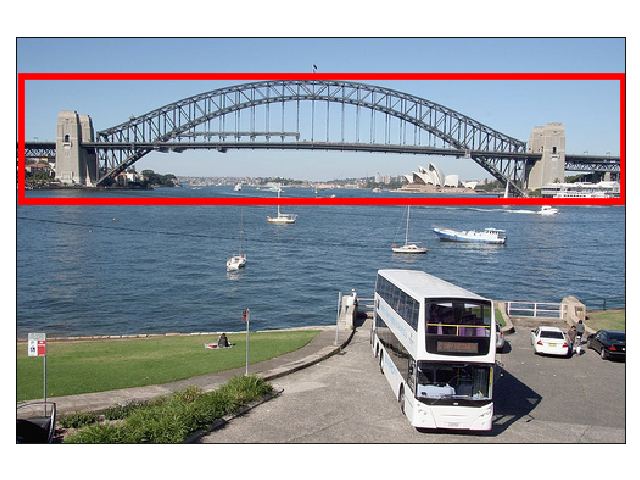
\includegraphics[width=0.9\linewidth]{figures/2341667_2006329_singleton_obj.png}} bridge (35)  &
				\raisebox{-\totalheight}{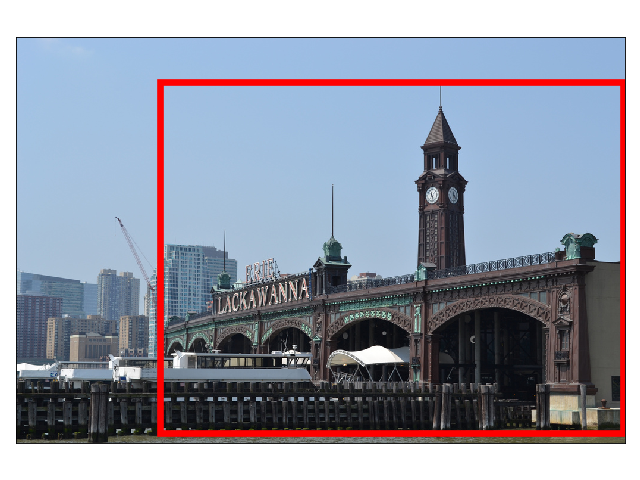
\includegraphics[width=0.9\linewidth]{figures/1592509_1610006_singleton_obj.png}} bridge (20),  \underline{building} (11)  &
				\raisebox{-\totalheight}{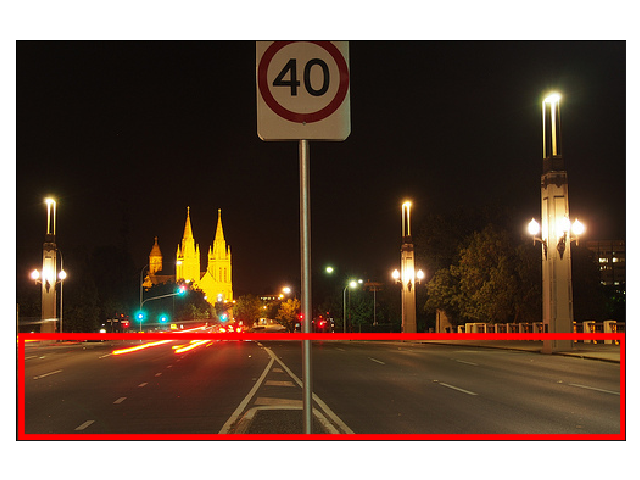
\includegraphics[width=0.9\linewidth]{figures/2384683_1306430_singleton_obj.png}} street (16), road (15), bridge (3) &
				\raisebox{-\totalheight}{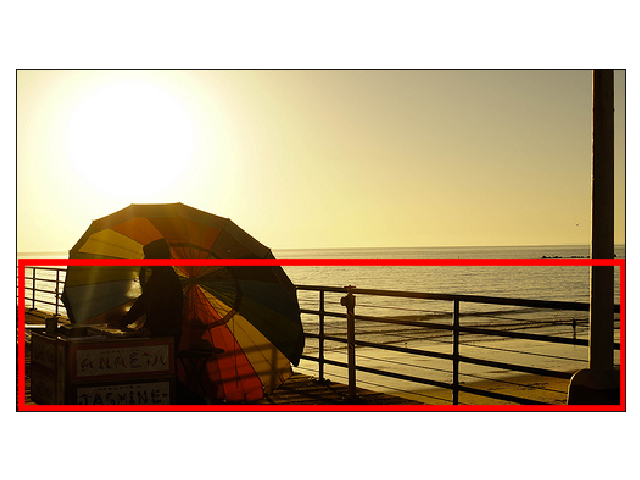
\includegraphics[width=0.9\linewidth]{figures/2412972_3494120_singleton_obj.png}} pier (6), railing (5), dock (5), bridge (5), fence (4), rail (3), boardwalk (3) &
				\raisebox{-\totalheight}{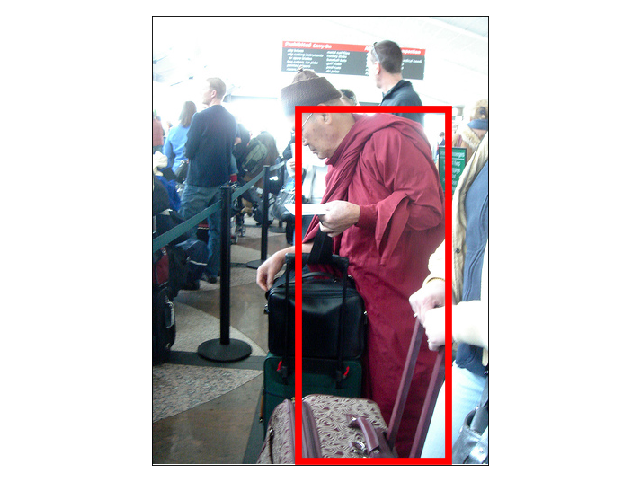
\includegraphics[width=0.9\linewidth]{figures/2334612_2838713_supercat_unique.png}}  robe (11), jacket (7), clothes (6), bag (3), dress (2), man (2) &
				\raisebox{-\totalheight}{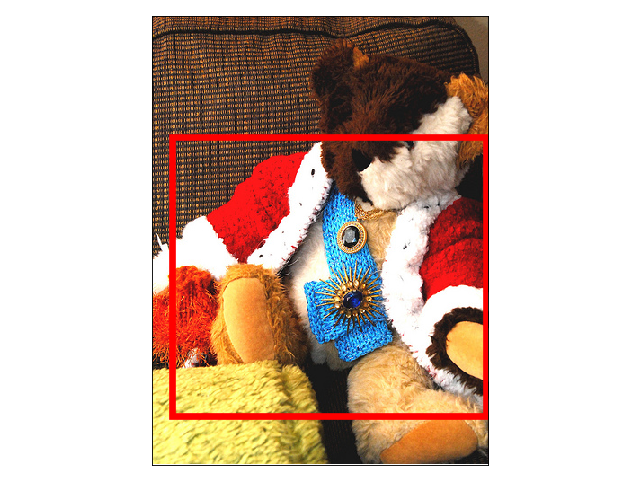
\includegraphics[width=0.9\linewidth]{figures/2340041_2137546_supercat_ambiguous.png}} jacket (10), \underline{sweater} (9), coat (3), doll (3), toy (3), \underline{shirt} (2), bear (2), robe (2) [stuffed animal (1)]\\
				%
				\rowcolor{lightgray}
				\textit{bridge}, arch, sky, structure, walkway
				& \textit{building}, \textit{bridge}, sky, structure, church
				& \textit{street}, \textit{road}, highway, intersection, pavement
				& \textit{railing}, water, \textit{pier}, ocean, \textit{fence}, deck, \textit{dock} 
			         & \textit{man}, shirt, person, \textit{robe}, coat, \textit{jacket}%, woman, outfit, clothes, clothing
				& teddy bear, \textit{bear}, dog, \textit{toy}, \textit{stuffed animal}, blanket, toys
\\ 
				%
				% 
				\multicolumn{4}{c|}{\textbf{VG: bed}} & \multicolumn{2}{c}{\textbf{VG: batter}}\\ 
				\raisebox{-\totalheight}{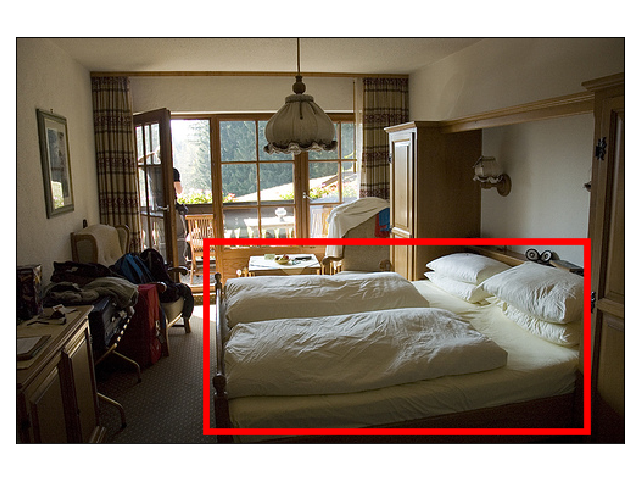
\includegraphics[width=0.9\linewidth]{figures/2321254_3438076_singleton_obj.png}} bed (36)  &
				\raisebox{-\totalheight}{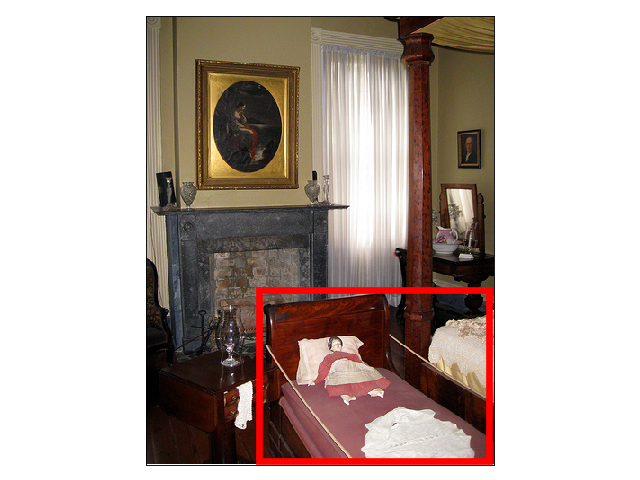
\includegraphics[width=0.9\linewidth]{figures/2324306_3412337_singleton_obj.png}}  bed (16), bench (6), crib (5) &
				\raisebox{-\totalheight}{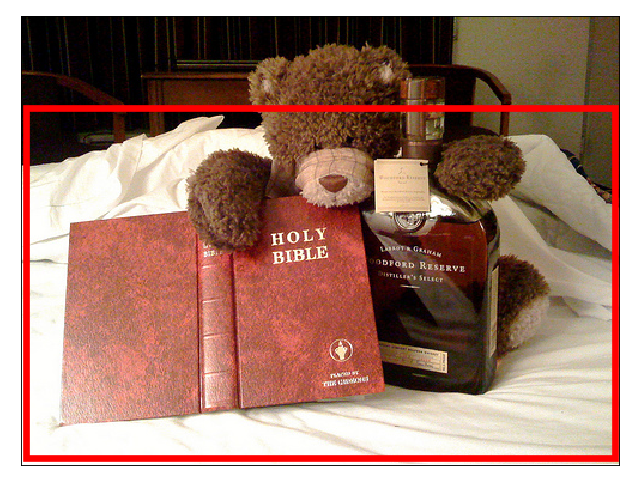
\includegraphics[width=0.9\linewidth]{figures/2342811_3485104_singleton_obj.png}}  bed (17), book (6), table (4), toy (3), bible (2), doll (2) & 
				\raisebox{-\totalheight}{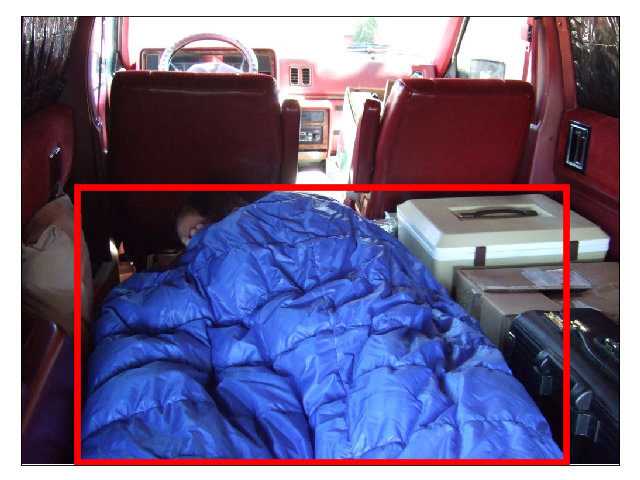
\includegraphics[width=0.9\linewidth]{figures/498222_3135415_singleton_obj.png}} bed (12), sleeping bag (9), blanket (7), bed sheet (5) &
				\raisebox{-\totalheight}{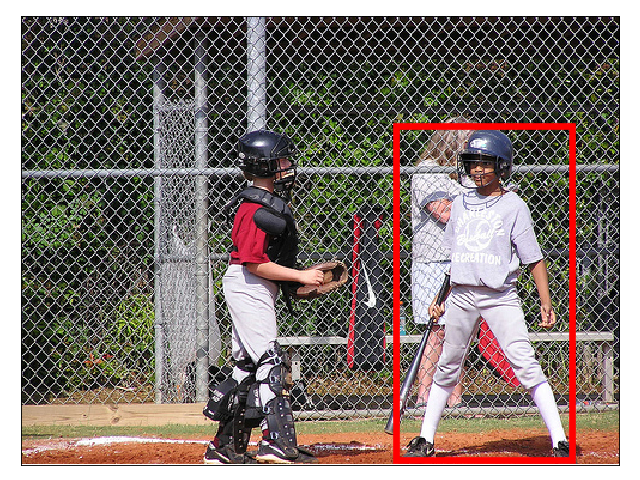
\includegraphics[width=0.9\linewidth]{figures/2398907_2901496_singleton_obj.png}}  boy (7), helmet (5), \underline{baseball player} (4), \underline{player} (4), man (3), child (3), batter (3), dress (2), kid (2)&
				\raisebox{-\totalheight}{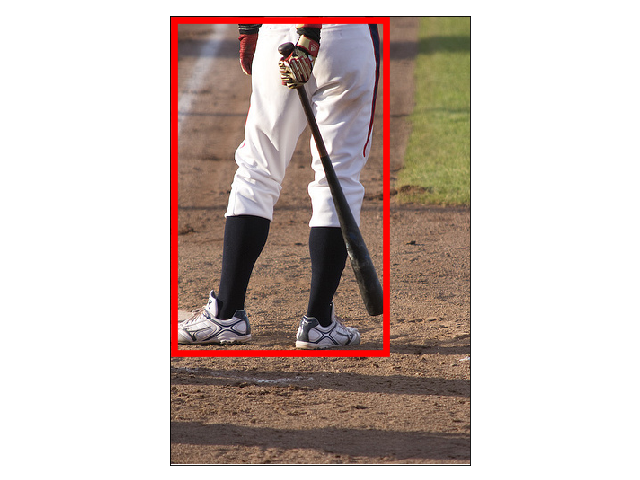
\includegraphics[width=0.9\linewidth]{figures/2337552_957263_singleton_obj.png}} pants (6), \underline{player} (5), shoe (4), bat (4), \underline{person} (4), legs (4), \underline{baseball player} (3), hitter (2)\\ \\ 
				%
				\rowcolor{lightgray}
				\textit{bed}, beds, sheets, frame, sheet
				& \textit{bed}, table, bed frame, sofa, couch
				& \textit{bed}, sheet, sheets, blanket, comforter, cover
				& \textit{bed}, comforter, \textit{blanket}, cover, sheet 
				& \textit{boy}, \textit{player}, \textit{batter}, \textit{kid}, girl, \textit{child}, \textit{baseball player}, person, uniform
				& \textit{player}, batter, \textit{person}, man, uniform, boy, \textit{baseball player}, dirt \\  
				%
				% 
%				\multicolumn{4}{c}{\textbf{VG: batter}}\\
%				\raisebox{-\totalheight}{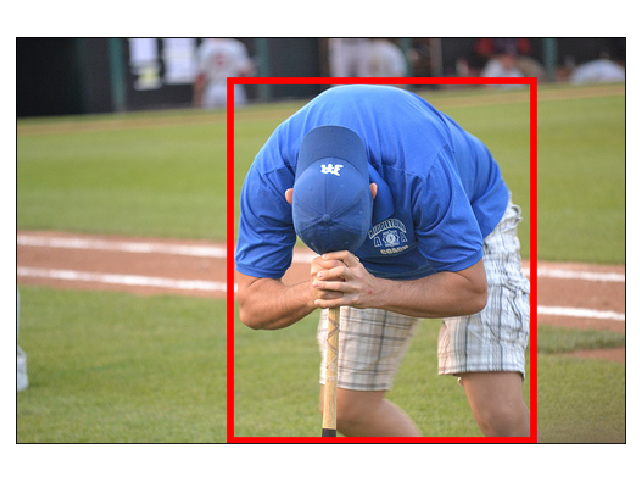
\includegraphics[width=0.9\linewidth]{figures/2372219_2683892_supercat_unique.png}} man (24), cap (5), \underline{person} (3), \underline{baseball player} (2) &
%				\raisebox{-\totalheight}{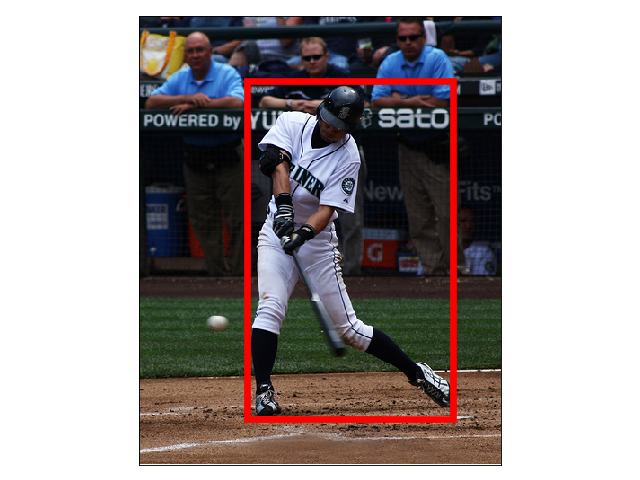
\includegraphics[width=0.9\linewidth]{figures/2394377_464684_singleton_obj.png}} man (13), \underline{baseball player} (7), batter (5), \underline{player} (3), helmet (2) [player (1)]&
%				\raisebox{-\totalheight}{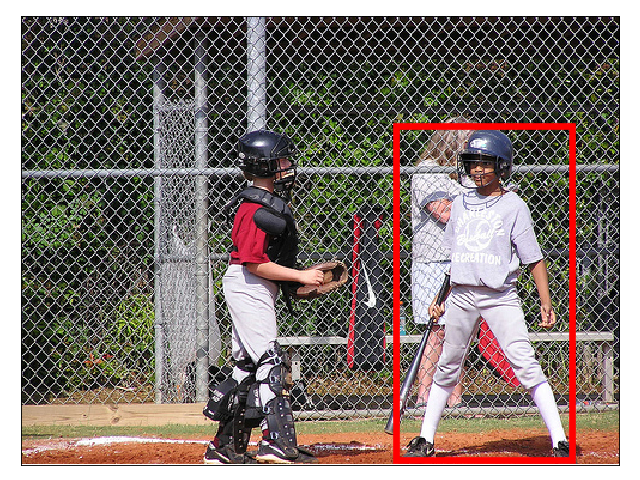
\includegraphics[width=0.9\linewidth]{figures/2398907_2901496_singleton_obj.png}}  boy (7), helmet (5), \underline{baseball player} (4), \underline{player} (4), man (3), child (3), batter (3), dress (2), kid (2)&
%				\raisebox{-\totalheight}{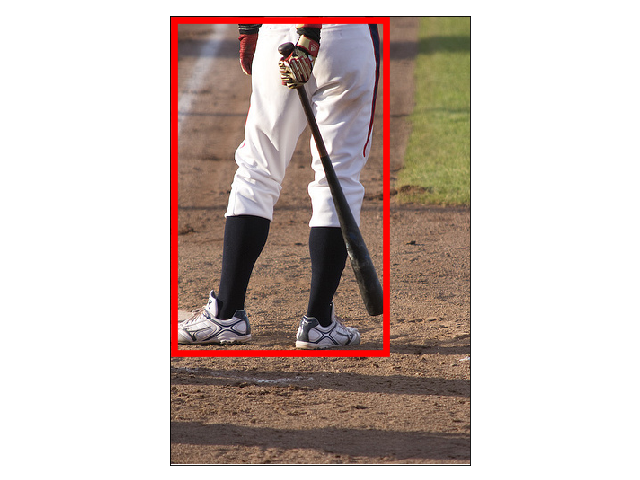
\includegraphics[width=0.9\linewidth]{figures/2337552_957263_singleton_obj.png}} pants (6), \underline{player} (5), shoe (4), bat (4), \underline{person} (4), legs (4), \underline{baseball player} (3), hitter (2)\\ 
%				%
%				\rowcolor{lightgray}
%				\textit{man}, player, \textit{person}, shirt, guy
%				& \textit{player}, \textit{batter}, \textit{man}, \textit{baseball player}, uniform
%				& \textit{boy}, \textit{player}, \textit{batter}, \textit{kid}, girl, \textit{child}, \textit{baseball player}, person, uniform
%				& \textit{player}, batter, \textit{person}, man, uniform, boy, \textit{baseball player}, dirt \\ 
				%
				% 
%				\multicolumn{4}{c}{\textbf{VG: robe}}\\
%				\raisebox{-\totalheight}{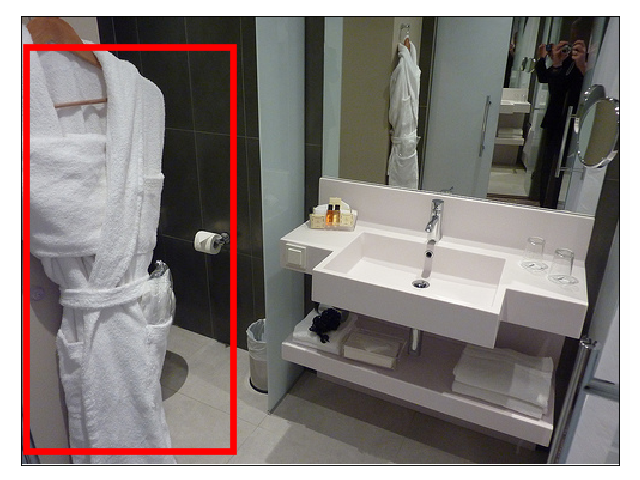
\includegraphics[width=0.9\linewidth]{figures/2373180_2333161_singleton_obj.png}} robe (27), \underline{bathrobe} (5) &
%				\raisebox{-\totalheight}{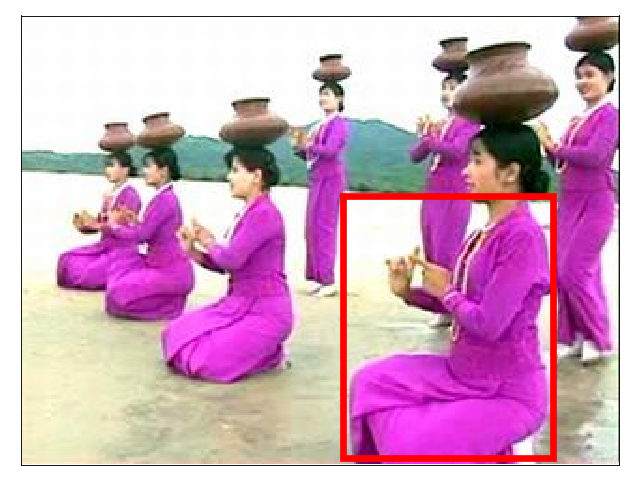
\includegraphics[width=0.9\linewidth]{figures/160_1058761_supercat_unique.png}} dress (30), uniform (2) &
%				\raisebox{-\totalheight}{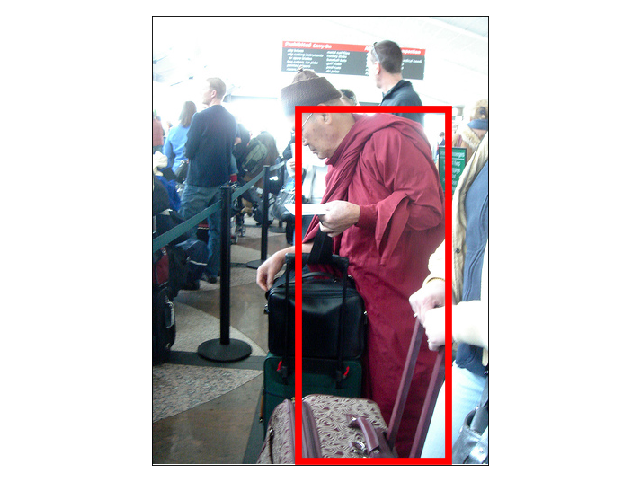
\includegraphics[width=0.9\linewidth]{figures/2334612_2838713_supercat_unique.png}}  robe (11), jacket (7), clothes (6), bag (3), dress (2), man (2) &
%				\raisebox{-\totalheight}{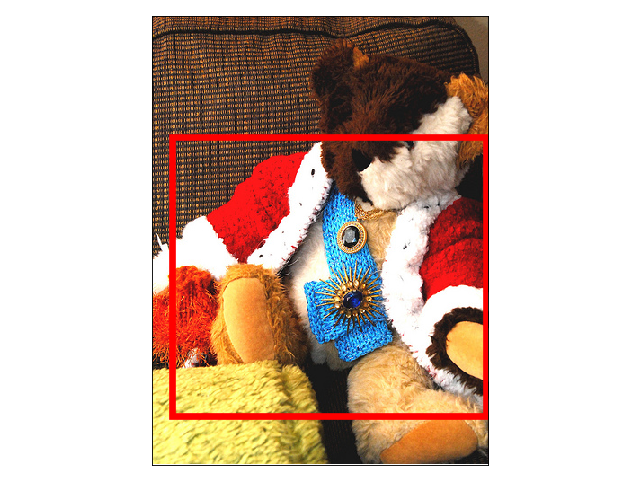
\includegraphics[width=0.9\linewidth]{figures/2340041_2137546_supercat_ambiguous.png}} jacket (10), \underline{sweater} (9), coat (3), doll (3), toy (3), \underline{shirt} (2), bear (2), robe (2) [stuffed animal (1)]\\ 
%				%
%				\rowcolor{lightgray}
%				woman, outfit, dress, girl, suit
%				& woman, outfit, \textit{dress}, girl, suit
%				& \textit{man}, shirt, person, \textit{robe}, coat, \textit{jacket}%, woman, outfit, clothes, clothing
%				& teddy bear, \textit{bear}, dog, \textit{toy}, \textit{stuffed animal}, blanket, toys
%				%, stuffed animals \\ 
%				%
%				% 				
			\end{tabular}
		}
	\end{minipage}
	\caption{Examples for instances of \vgenome synsets with low and high agreement in ManyNames. 
		First row: responses in MN, names that have a hierarchical relation to the \vgenome synset in WordNet are underlined.
	Second row (gray): top name prediction by bottom up, names which match a MN response are in italics.}
	\label{fig:ex-high-low-agreement}
\end{figure*}



%\begin{figure*}
\begin{minipage}[b]{0.5\linewidth}
{\footnotesize
\setlength{\tabcolsep}{1pt}
\begin{tabular}{p{4cm}|p{4cm}|p{4cm}|p{4cm}}
%\textbf{desk} &  \raisebox{-\totalheight}{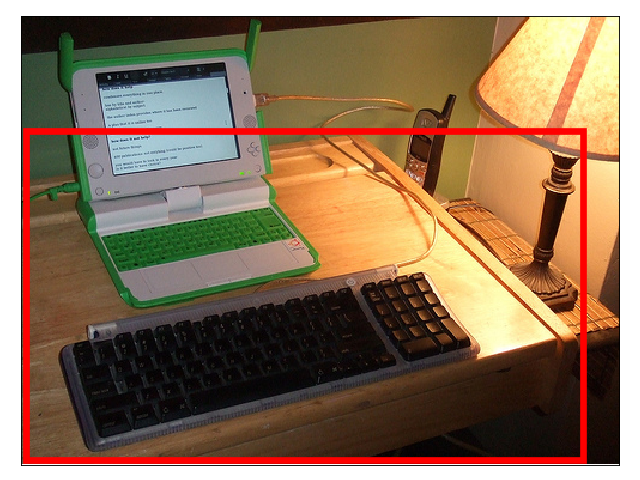
\includegraphics[width=0.9\linewidth]{figures/2320949_1048853_singleton_obj.png}} MN: keyboard  &
%\raisebox{-\totalheight}{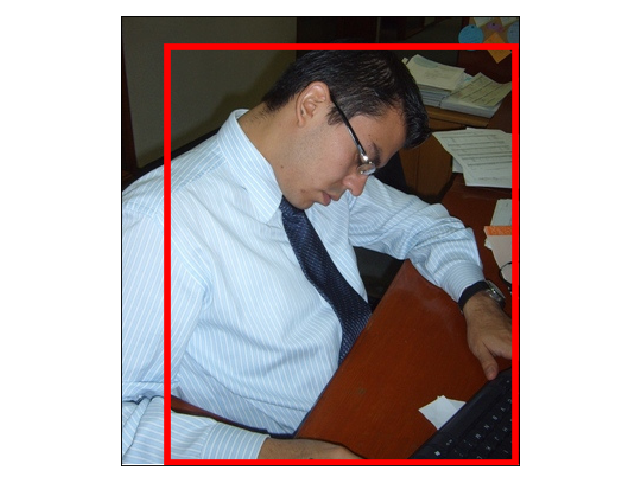
\includegraphics[width=0.9\linewidth]{figures/2343219_926143_supercat_unique.png}}  MN: desktop &
%\raisebox{-\totalheight}{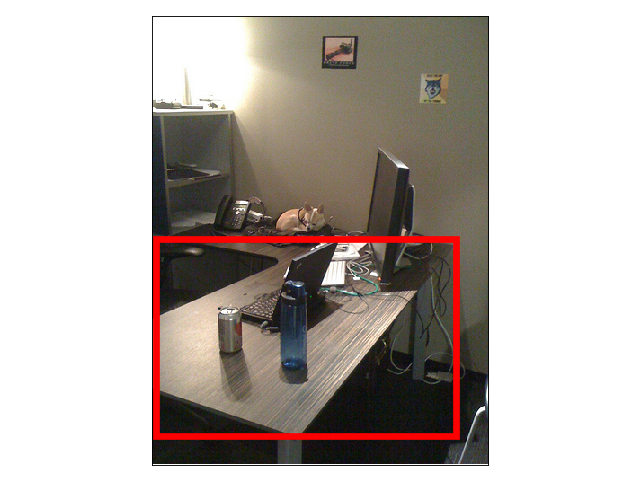
\includegraphics[width=0.9\linewidth]{figures/2354847_1742687_seed_ambiguous.png}} MN: computer \\
%\textbf{bench} &  \raisebox{-\totalheight}{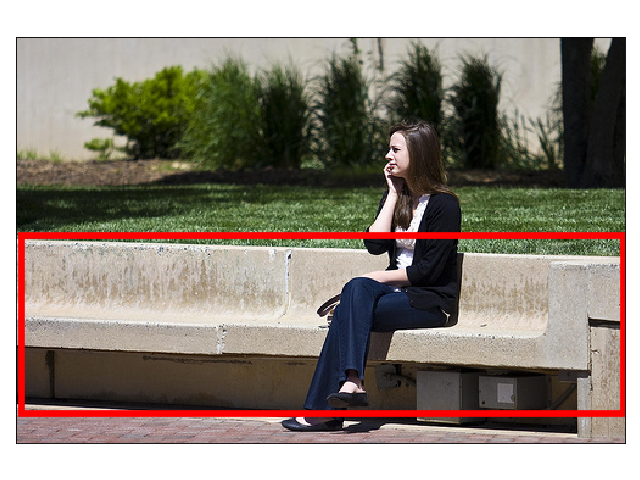
\includegraphics[width=0.9\linewidth]{figures/2350360_1042111_supercat_unique.png}} MN: table  &
%\raisebox{-\totalheight}{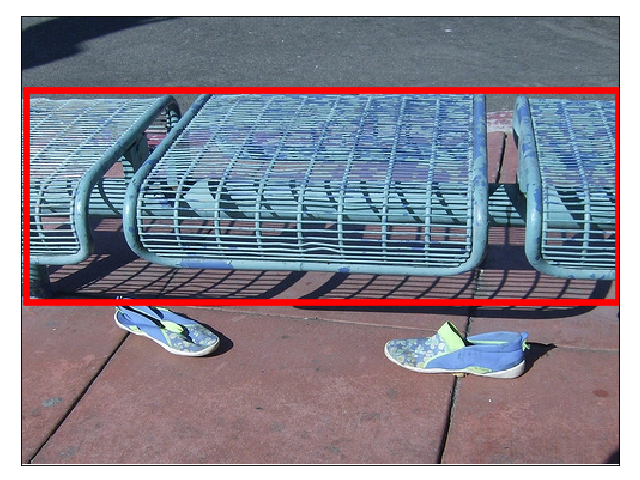
\includegraphics[width=0.9\linewidth]{figures/2389358_1261752_singleton_obj.png}}  MN: seat &
%\raisebox{-\totalheight}{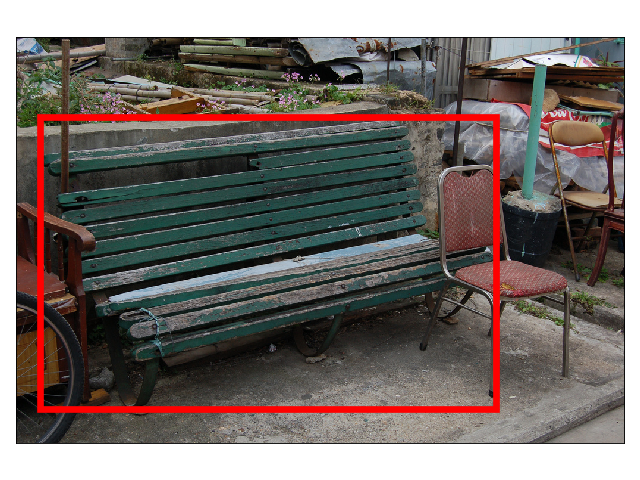
\includegraphics[width=0.9\linewidth]{figures/1593011_2063521_singleton_obj.png}} MN: wood \\
\multicolumn{4}{c}{\textbf{VG: sandwich}}\\
 \raisebox{-\totalheight}{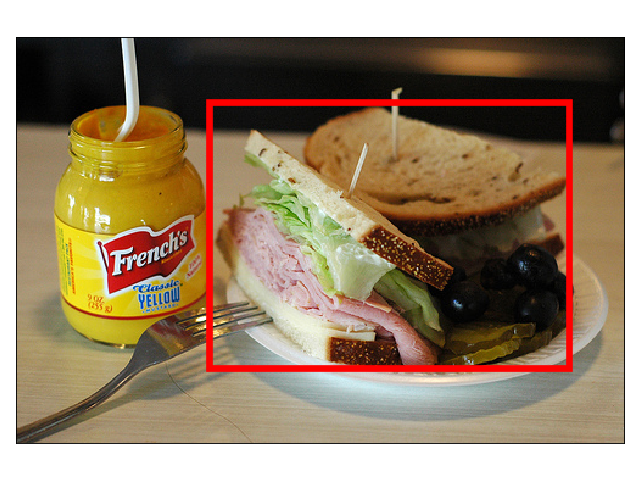
\includegraphics[width=0.9\linewidth]{figures/2339876_3928476_supercat_unique.png}} sandwich (34) &
\raisebox{-\totalheight}{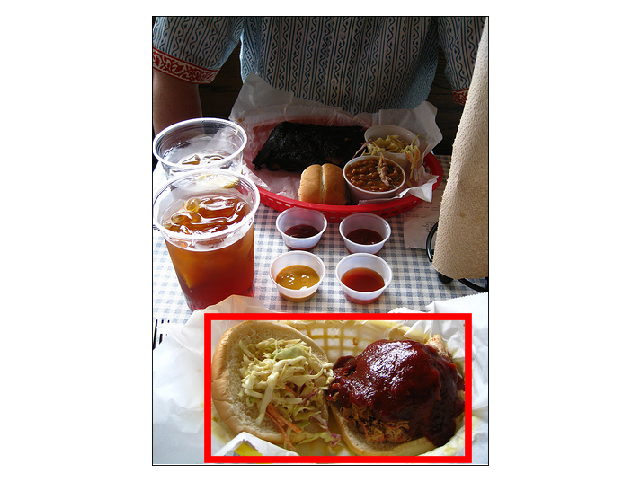
\includegraphics[width=0.9\linewidth]{figures/2379889_1353176_supercat_unique.png}}  sandwich (15), basket (6), \underline{food} (5), burger (2),  \underline{hamburger} (2),  \underline{meal} (2) &
\raisebox{-\totalheight}{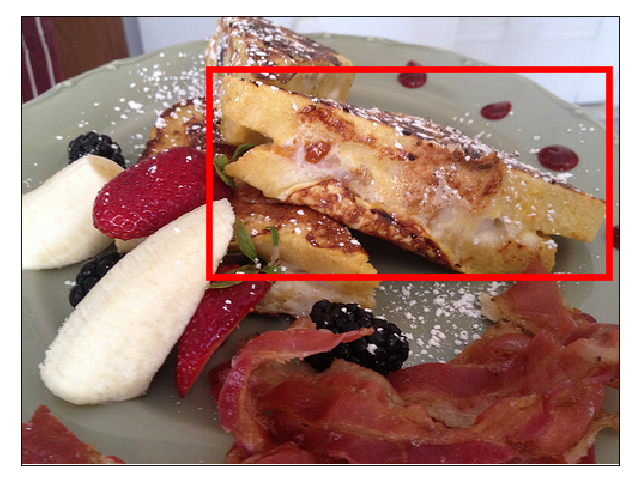
\includegraphics[width=0.9\linewidth]{figures/2394266_465678_singleton_obj.png}} \underline{food} (10), sandwich (8), toast (5), french toast (4), dessert (2), breakfast (2) &
\raisebox{-\totalheight}{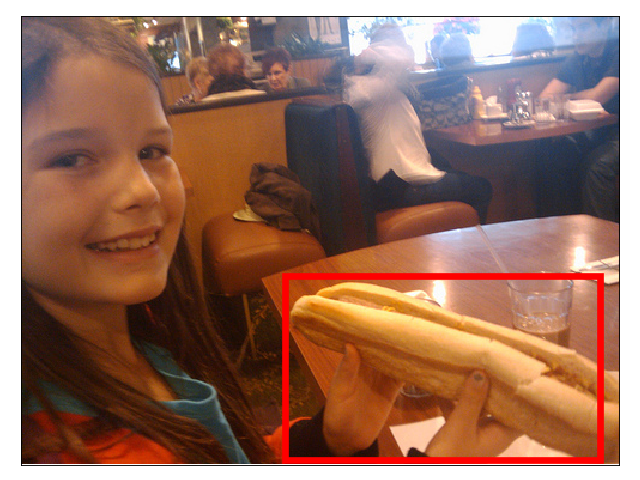
\includegraphics[width=0.9\linewidth]{figures/2386509_681763_supercat_unique.png}} hotdog (14), \underline{food} (7), bun (4), sandwich (3),  \underline{bread} (2)\\ 
\multicolumn{4}{c}{\textbf{VG: bridge} }\\ 
\raisebox{-\totalheight}{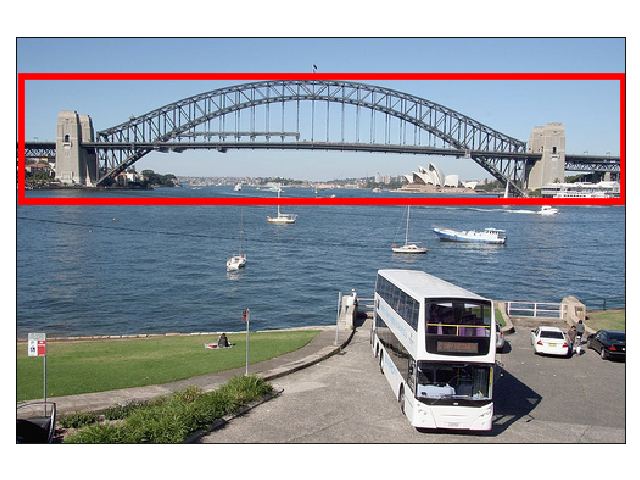
\includegraphics[width=0.9\linewidth]{figures/2341667_2006329_singleton_obj.png}} bridge (35)  &
\raisebox{-\totalheight}{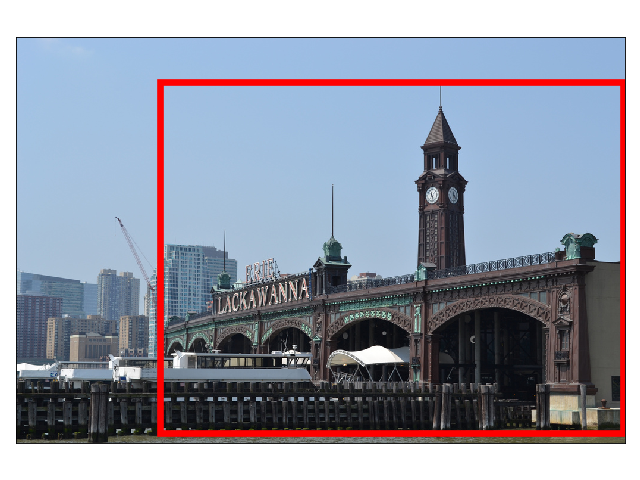
\includegraphics[width=0.9\linewidth]{figures/1592509_1610006_singleton_obj.png}} bridge (20),  \underline{building} (11)  &
\raisebox{-\totalheight}{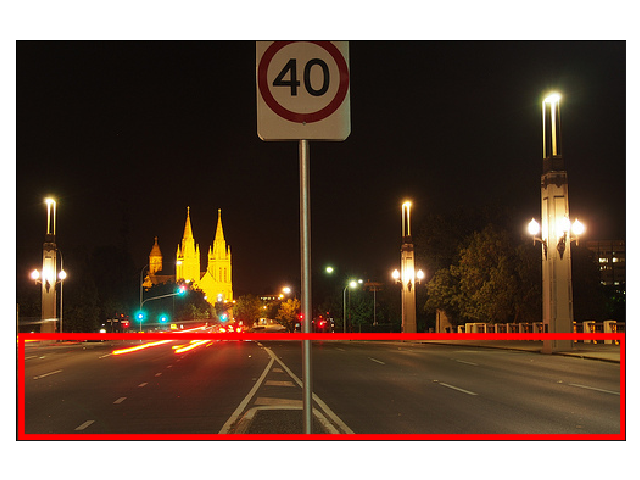
\includegraphics[width=0.9\linewidth]{figures/2384683_1306430_singleton_obj.png}} street (16), road (15), bridge (3) &
\raisebox{-\totalheight}{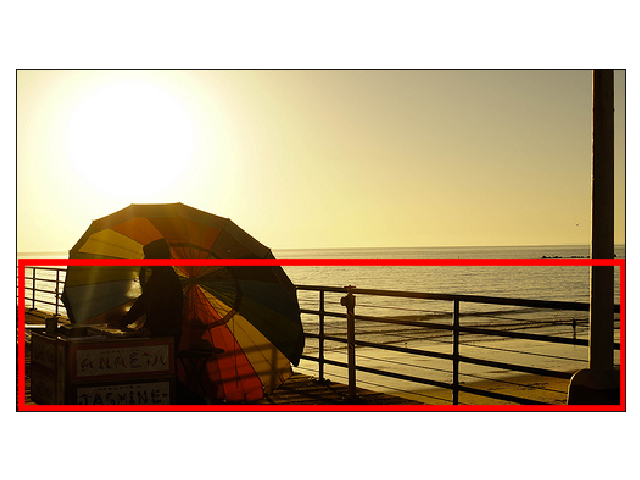
\includegraphics[width=0.9\linewidth]{figures/2412972_3494120_singleton_obj.png}} pier (6), railing (5), dock (5), bridge (5), fence (4), rail (3), boardwalk (3)\\ 
\multicolumn{4}{c}{\textbf{VG: bed}}\\ 
\raisebox{-\totalheight}{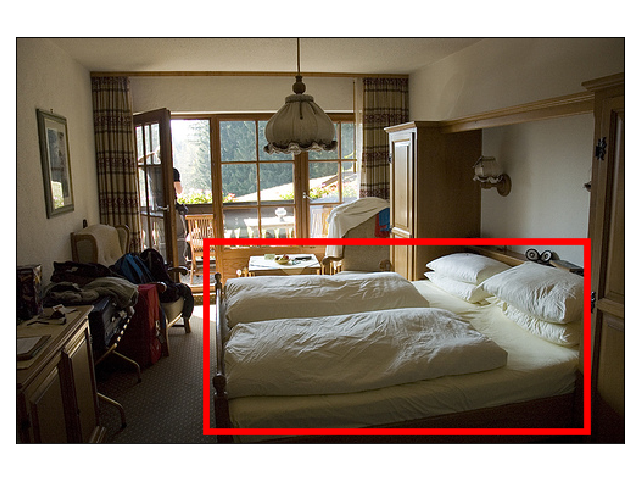
\includegraphics[width=0.9\linewidth]{figures/2321254_3438076_singleton_obj.png}} bed (36)  &
\raisebox{-\totalheight}{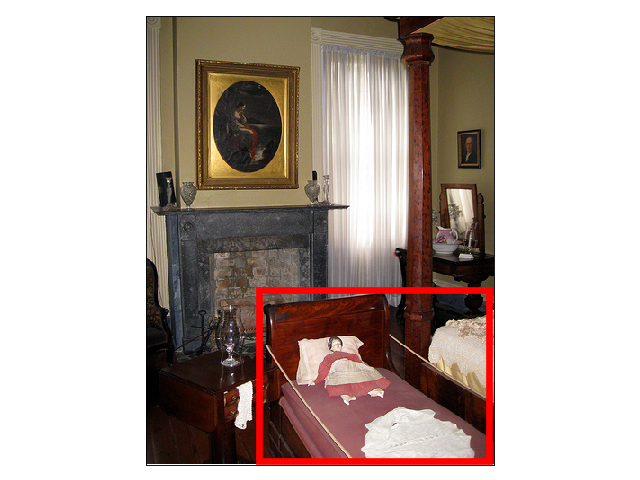
\includegraphics[width=0.9\linewidth]{figures/2324306_3412337_singleton_obj.png}}  bed (16), bench (6), crib (5) &
\raisebox{-\totalheight}{\includegraphics[width=0.9\linewidth]{figures/2342811_3485104_singleton_obj.png}}  bed (17), book (6), table (4), toy (3), bible (2), doll (2) & 
\raisebox{-\totalheight}{\includegraphics[width=0.9\linewidth]{figures/498222_3135415_singleton_obj.png}} bed (12), sleeping bag (9), blanket (7), bed sheet (5)\\ 
\multicolumn{4}{c}{\textbf{VG: batter}}\\
\raisebox{-\totalheight}{\includegraphics[width=0.9\linewidth]{figures/2372219_2683892_supercat_unique.png}} man (24), cap (5), \underline{person} (3), \underline{baseball player} (2) &
  \raisebox{-\totalheight}{\includegraphics[width=0.9\linewidth]{figures/2394377_464684_singleton_obj.png}} man (13), \underline{baseball player} (7), batter (5), \underline{player} (3), helmet (2) &
\raisebox{-\totalheight}{\includegraphics[width=0.9\linewidth]{figures/2398907_2901496_singleton_obj.png}}  boy (7), helmet (5), \underline{baseball player} (4), \underline{player} (4), man (3), child (3), batter (3), dress (2), kid (2)&
\raisebox{-\totalheight}{\includegraphics[width=0.9\linewidth]{figures/2337552_957263_singleton_obj.png}} pants (6), \underline{player} (5), shoe (4), bat (4), \underline{person} (4), legs (4), \underline{baseball player} (3), hitter (2)\\ 
\multicolumn{4}{c}{\textbf{VG: robe}}\\
\raisebox{-\totalheight}{\includegraphics[width=0.9\linewidth]{figures/2373180_2333161_singleton_obj.png}} robe (27), \underline{bathrobe} (5) &
  \raisebox{-\totalheight}{\includegraphics[width=0.9\linewidth]{figures/160_1058761_supercat_unique.png}} dress (30), uniform (2) &
\raisebox{-\totalheight}{\includegraphics[width=0.9\linewidth]{figures/2334612_2838713_supercat_unique.png}}  robe (11), jacket (7), clothes (6), bag (3), dress (2), man (2) &
\raisebox{-\totalheight}{\includegraphics[width=0.9\linewidth]{figures/2340041_2137546_supercat_ambiguous.png}} jacket (10), \underline{sweater} (9), coat (3), doll (3), toy (3), \underline{shirt} (2), bear (2), robe (2)\\ 
\end{tabular}
}
\end{minipage}
 \caption{Examples for different instances of \vgenome synsets with low and high agreement in ManyNames data set, names that have a hierarchical relation to the \vgenome synset in WordNet are underlined}
\label{fig:ex-high-low-agreement}
\end{figure*}

%\gbt{The non-canon. VG names suggest that people prefer more general names (``car $>$ sedan'', ``horse $>$ pony'', ``tie $>$ necktie''). Could be due to lexical availability (more general \ra more frequent \ra more available). This could be verified (using frequency). Hypothesis: In cases where top name != VG, the VG name is less general. Could be also a more general hypothesis: see if people prefer more frequent names in general.}
%\cs{@Table~\ref{tab:qual} (just wrt presentation) The most interesting blocks are 2 and 3 (canonical VG with min agr.; non-canonical with max agr.)}

\subsection{Discussion}
\label{subsec:discuss}

% gbt: I moved the following sentence to the Conclusion section. To determine: what parts of this discussion stay here, what go to the conclusion.
% The object naming variation attested in the ManyNames dataset offers new challenges and perspectives, both for practical modeling approaches in Language \& Vision as well as for theoretical work in (Psycho-)linguistics.

The answer to our question, \textit{do objects in real-world images have a canonical name?} is nuanced. 
Our data indeed indicates a tendency for particular instances marked by bounding boxes to elicit a single consistent name across subjects, which is in line with existing theoretical research on object naming and categorization \cs{ok??}. 
However, we show that there is also consistent variation in naming, and even high variability in agreement across instances within the same class or domain. 
The latter suggests that there are specific visual characteristics of either the object itself or the visual context in which it appears that trigger variation. \cs{With prototypical pictures (see Figure\ \ref{fig:picture_naming}), as done in traditional studies, this observation would not be possible. (??)} 
%For theoretical research, w
We moreover find that much of the variation in object naming cannot be explained by adopting a traditional taxonomy-driven and hierarchical view, which has been dominant in the literature.

Our ManyNames dataset can be used for both, theoretical and practical research. 
Specifically, it provides a means 
(i) to study how different people would name the same object (image region) \cs{"visual awareness" would fit in here}, and, given a specific name, estimate its degree of preference, which might vary substantially across different instances of a class, and   
%assess the extent to which different speakers prefer that name, which might vary substantially across different instances of a class, and to 
(ii) to obtain a set of possible names for individual objects, as well as available lexical alternatives for specific names, which again might vary strongly across instances and often cannot be retrieved from existing taxonomies like WordNet. 

As far as research in L\&V and Computer Vision is concerned, our findings are reason to question the appropriateness of the standard, single-label approach in visual object naming and categorization methods. 
Even the assumption that there at least exists a canonical name
%,\ i.e.,\ a  name on which the majority of people would agree 
 for individual visual objects (localized by bounding boxes) is disputable (cf.\ the high standard deviation in terms of the relative frequency of an instance's top response (column \%top, Table~\ref{tab:agree}), and the average mismatch of $27\%$~between the instances' top response and their VG name (\mbox{top=VG})\cs{a bit redundant now}).
%
The ability to distinguish incorrect object names from name alternatives is essential for visual object understanding, though. 
It would be desirable to explicitly assess models towards their ability to account for naming variants of an instance (e.g.,~in how far are the top N predicted names valid alternatives, such as, dog, animal, pet vs. dog, animal, hat?). 
%
The criticism on the use of single "ground truth" labels is not new, but %to our knowledge 
as we outlined in Section\ \ref{sec:relwork}, previous work has focused on the determination of canonical names, or on "granularity-aware" models, where naming variants are hierachically related. 
\cs{check that this is in related work: previous work has focused on the determination of canonical names (e.g.,~\newcite{Ordonez:2016}; Mathews et al REF), or on "granularity-aware" models, where naming variants are hierachically related (e.g.,~\newcite{wang2014poodle, peterson2018learning}; Ristin et al., 2015 REF, and the references therein).}
%
% \textit{training} of classifiers with multiple labels to improve image classification model depicting multiple objects (e.g.,~Wang et al., 2016 REF)
% Wang et al.: ". The hypothesis is that by modeling the variation in granularity levels for different concepts, we can gain a more informative insight as to how the output of image annotation systems can relate to how a person describes what he or she perceives in an image, and consequently produce image annotation systems that are more human-centric."
% @related work
%[For example, \newcite{peterson2018learning} train CNN classifiers on objects with multiple labels which stand in a hierarchical relation (e.g., dog, animal) in order to learn better visual representations which capture the hierarchical structure of a taxonomy. \cs{remove or move to related work? also sentence to Ordonez}]
%\footnote{Other work used training data with multiple labels per image to improve image classification performance on images with multiple objects (e.g.,~Wang et al., 2016 REF). \cs{maybe remove, since it is not that relevant?}}
%
%
% peterson2018learning: discuss the bias introduced into learned representations by training on data of  single label annotations ("labels cut arbitrarily across natural psychological taxonomies, e.g., dogs are separated into breeds but never categorized as dogs"). 
%
However, given the fact that naming variants are often not recoverable by hierarchical relations, a taxonomic hierarchy is only limited in its use to distinguish automatically a truly false prediction (e.g.,\ \textsl{plate}) from a (possibly context-specific) valid alternative (e.g.,\ \textsl{basket}) to the single "ground truth" in a dataset (e.g.,\ \textsl{sandwich}). 
For the same reason, even fine-grained recognition models (as those trained on ILSVRC REF) cannot be expected to be able to simply infer the recognition of more general classes.
%since we found that many name alternatives are not hierarchically related to the VG name, there is only limited use of, e.g., a taxonomic hierarchy, to distinguish automatically a "truly" false prediction (e.g.,\ \textsl{plate}) from a (possibly context-specific) valid alternative (e.g.,\ \textsl{basket}) to the single "ground truth" in a dataset (e.g.,\ \textsl{sandwich}). 
\cs{also distributional similarity? Remember that we looked into this for the checkpoint and did not find a clear similarity threshold/pattern} 
%

\cs{?: Say something about type disagreements on class-level, after having written the results discussion.}
%

\cs{Ah, we still should have a comparison model with above argumentation :/.}
%
As a use-case study, in Section\ \ref{sec:modeling}, we will treat ManyNames as evaluation data and assess whether an existing SOTA model can account for the naming variants of individual objects. 

\iffalse
*********
Existing large-scale collections of labels or names of objects in L\&V provide simple annotations of individual objects with canonicalized name sets.
When humans agree only around 70\% of the cases in how to name an object, it is not clear that the data can be taken as a gold standard in multi-label classification setting, as is commonly done in Computer Vision.
% At the same time, compared to annotation and modeling frameworks in Computer Vision that frame the problem as an object labeling task, our data shows a much lower agreement than what should be expected if object names were indeed entirely canonical,
See e.g.\ the ResNet which achieves a top-1 error rate of 25\% on ILSVRC 2015. \gbt{It is not clear to me what this means: what kind of data is this? how does this result relate to our point? -- @Carina, expand?}
\fi

\gbt{I couldn't follow the discussion in the following pargraph. Do you think it's subsumed by the one above? Can we remove it?} 
Given that we find much lower agreement on object class-level than on an instance-level, one might argue for using very fine-grained object annotations to remedy this problem. 
However, the fact that naming variants are often not recoverable by hierarchical relations suggest that even fine-grained recognition models cannot be expected to be able to simply infer recognition of more general classes (e.g., ILSVRC synset). Thus, neither simple multi-label classification nor more advance hierarchical approaches to object recognition seem to be well designed for capturing natural naming phenomena comprising cross-classification, metonymy and potentially other sources of variation.

%What does this discrepancy between the instance-level and category-level agreement in VisualGenome and ManyNames naming choices mean? 
%First of all, it suggests that the same original VisualGenome name can trigger very different variants depending on the visual instance, leading to a drastic increase of variants elicited for categories as compared to instances.
%Second, this clearly shows that annotators in VG do not generally annotate the most canonical name \cs{but they don't annotate the name, but the description} and that many names annotated for objects in VG do not correspond to the overall most preferred variant. \sz{think more ...}
%\gbt{I don't think we can conclude this second part -- we do have the 70\% top=VG figure that says that VG annotators annotate the most canonical name. What this suggests to me is that instance-level properties are more important than category-level properties, somehow.

%Why is naming more flexible in certain domains than in others? \gbt{Hypothesis: expectation: little variation - hypernymy at most, more variation <-> more affordances <-> more varied relationships.}

%\cs{@Table~\ref{tab:agree} I still think that we could also have \%\ top with $N>1$ to give an idea as to how useful the data is for the people interested in using it for, e.g., model evaluation. For that, it is clear that crowdsourcing is noisy and before using it some outlier removal needs to be made.}

% \subsection{Entry-level names and preference orders....}

% \sz{an interesting example:} In our data set, there are 24 images where \textit{penguin} has been used, so we know that the object is a \textit{penguin}. For 50\% of these images, annotators still prefer \textit{bird} as the most common name. According to the theory of entry-level categories, this should not happen. People should always prefer \textit{penguin} over \textit{bird}. 

% \sz{how can we analyze this quantitatively?}

% \begin{itemize}
% \item lettuce -- salad
% \item fruit -- food
% \item man -- catcher
% \item bowl --chili
% \item bowl -- diner \gbt{spelling mistake? should be dinner?} 
% \item burger -- meat
% \item statue -- animal (image shows statue of an animal)
% \item bottle -- alcohol
% \item donut --desert \gbt{spelling mistake? should be dessert?} 
% \item zebra -- stripes
% \item oven -- grill
% \end{itemize}


%%% Local Variables:
%%% mode: latex
%%% TeX-master: "main"
%%% End:


